\chapter{Introducción}

\section{Procesamiento del Lenguaje Natural}

Con el avance errático de la tecnología, el ser humano ha buscado formas no solo de solucionar 
problemas, sino también de resolverlos de la manera más eficiente posible utilizando 
el poder de cómputo de las computadoras. En particular, se ha buscado que estas 
pudieran reconocer y comprender el lenguaje utilizado por los seres humanos y 
realizar acciones en base al mismo. A partir de esta idea es donde nace un subcampo 
de la informática y la inteligencia artificial llamado procesamiento del lenguaje natural (NLP, por sus siglas en inglés).

El NLP permite que las computadoras y los dispositivos digitales reconozcan, comprendan y generen texto y habla al combinar la lingüística computacional, la modelación basada en reglas del lenguaje humano, junto al modelado estadístico, el aprendizaje automático y el aprendizaje profundo.

La investigación en NLP ha sido uno de los actores claves que han dado lugar a la era de la IA generativa, desde las habilidades comunicativas de los grandes modelos de lenguaje (LLMs) hasta la capacidad de ciertos modelos para poder generar imágenes a partir de una descripción escrita. El NLP ya forma parte de la vida cotidiana para muchos, alimentando motores de búsqueda, impulsando chatbots para servicio al cliente con comandos de voz, sistemas de GPS operados por voz y asistentes digitales en teléfonos inteligentes.

\subsection{Representación Vectorial de palabras}

Una de las primeras cuestiones que surgen cuando hablamos sobre NLP es como representar las palabras del lenguaje para que las computadoras sean capaces de reconocerlas y utilizarlas de manera eficiente. En un principio, uno estaría tentado de sugerir la idea más simple posible, y representar las palabras como comúnmente las observamos, como secuencias de caracteres. Sin embargo, es importante tener en cuenta que existe una cantidad inmensa de información extra fuera de estas cadenas de caracteres que nos permiten entender el significado de las mismas, como puede ser el contexto o la semántica de la propia palabra. Esto genera que utilizar texto plano para identificar estas palabras y alimentar a los modelos de NLP no lleve a buen puerto.

Para suplir estas falencias se crearon los llamados vectores de palabras, o \textit{word embeddings}, los cuales son representaciones numéricas de palabras en un espacio de alta dimensión. Cada palabra está representada por un vector y la posición de cada palabra en este espacio se determina por el contexto en el que aparece en los textos de entrenamiento. Así, palabras con significados similares tendrán vectores cercanos en este espacio. Incluso, complejizando estos \textit{embeddings}, se puede captar información para poder reconocer de manera correcta palabras que tienen más de un significado (palabras polisémicas). \parencite{liu2020surveycontextualembeddings}

\begin{figure}[H]
    \centering
    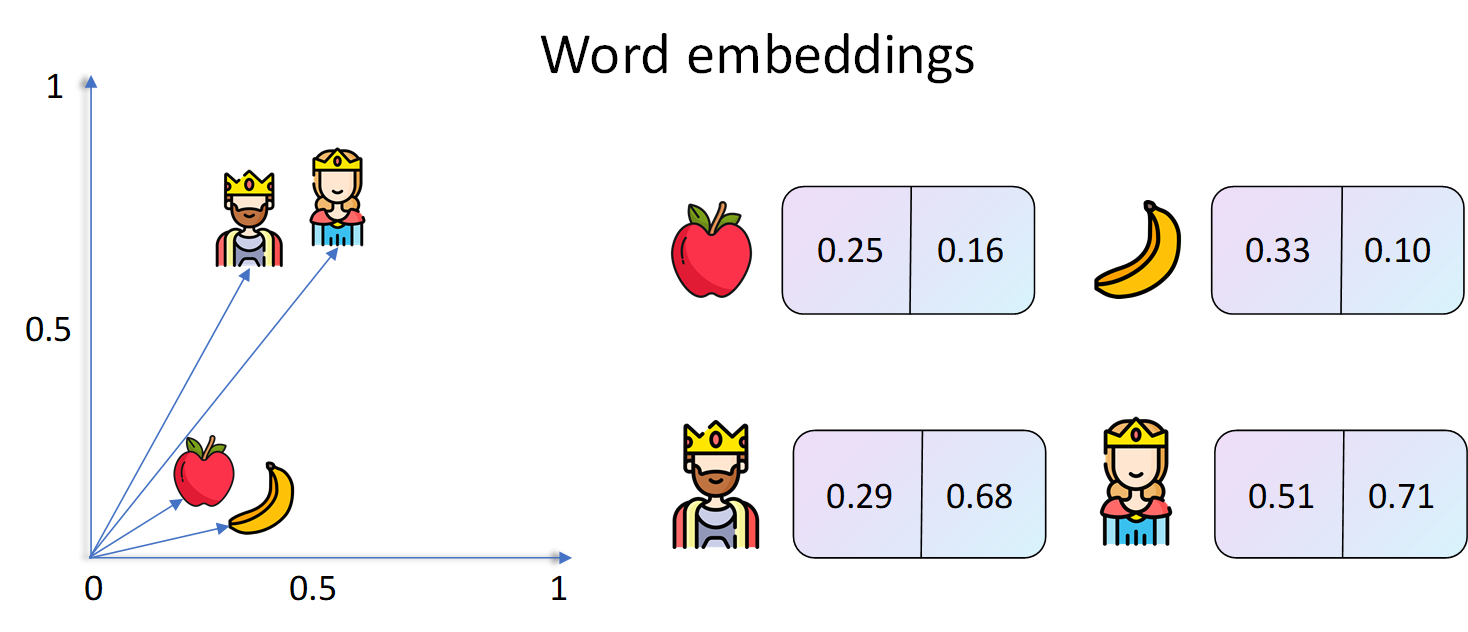
\includegraphics[width=1\textwidth]{imagenes/word_embeddings.png}
    \caption{Los vectores de palabras permiten asociar palabras mediante su cercanía dimensional, así palabras como rey o reina, o manzana y banana, se encuentran cerca en el plano.}
    \label{fig:word_embbeding}
\end{figure}

Las representaciones vectoriales de palabras han revolucionado tareas de procesamiento de lenguaje natural como la traducción automática, el análisis de sentimientos y la recuperación de información. \parencite{sentimentanalysisspanishtweets} Estas representaciones permiten a las computadoras entender el significado de las palabras y sus relaciones, lo que les permite realizar tareas lingüísticas complejas.

\subsubsection{Evaluación}

Diferentes modelos de \textit{word embeddings} generan representaciones vectoriales distintas. Sin embargo, existen algunas propiedades que todas estas representaciones deben buscar para considerarse útiles y de calidad \parencite{Wang_2019}:

\begin{itemize}
    \item No-Fusión: Los diferentes contextos locales alrededor de una palabra deben dar lugar a propiedades específicas de la palabra, como el plural o singular, los tiempos verbales, etc. Los modelos de \textit{word embeddings} deben ser capaces de discernir las diferencias en los contextos y codificar estos detalles en una representación significativa en el subespacio de la palabra. \parencite{yaghoobzadeh2016intrinsicsubspaceevaluationword}
    \item Robustez frente a la ambigüedad léxica: Deben estar representados todos los sentidos (o significados) de una palabra. Los modelos deben poder distinguir el sentido de una palabra a partir de su contexto y encontrar el embedding apropiado. \parencite{yaghoobzadeh2016intrinsicsubspaceevaluationword}
    \item Demostración de multifaceticidad: Los aspectos fonéticos, morfológicos, sintácticos y otras propiedades de una palabra deben contribuir a su representación final. Esto es importante ya que los modelos de palabras deberían generar representaciones significativas y quizás encontrar relaciones entre diferentes palabras. Por ejemplo, la representación de una palabra debería cambiar cuando se cambia el tiempo verbal o se añade un prefijo. \parencite{yaghoobzadeh2016intrinsicsubspaceevaluationword}
    \item Confiabilidad: Los resultados de un modelo de \textit{embeddings} de palabras deben ser confiables. Esto es importante ya que los vectores de palabras se inicializan aleatoriamente durante el entrenamiento. Incluso si un modelo crea representaciones diferentes del mismo conjunto de datos debido a la inicialización aleatoria, el rendimiento de varias representaciones debería ser consistente. \parencite{HellrichH17}
    \item Buena geometría: Un espacio de \textit{embeddings} debe estar correctamente distribuido. En términos generales, un conjunto pequeño de palabras frecuentes y no relacionadas debería distribuirse uniformemente en todo el espacio, mientras que un conjunto mayor de palabras raras debería agruparse alrededor de las palabras frecuentes. \parencite{GladkovaDrozd2016}
\end{itemize}

Por lo tanto, con estas propiedades en mente, se han definido varias formas de evaluar a los \textit{embeddings} resultantes de un modelo, utilizando tanto distintas tareas de NLP para evaluarlos (métodos extrínsecos) como tareas totalmente independientes a estas (métodos intrínsecos).

Uno de los métodos intrínsecos más usados es la distancia entre vectores. Al interpretar la distancia entre dos vectores como medida de similitud, se evalúa su correlación con la similitud semántica percibida por los humanos. El objetivo es medir qué tan bien las representaciones vectoriales de palabras capturan la noción de similitud percibida por los humanos y validar la hipótesis distribucional, donde el significado de las palabras está relacionado con el contexto en el que ocurren. \parencite{Wang_2019}

Un evaluador comúnmente utilizado para obtener esta métrica es la similitud coseno, definida por:

\[
\text{Similitud} = \frac{\mathbf{A} \cdot \mathbf{B}}{\|\mathbf{A}\| \|\mathbf{B}\|}
\]

Donde \( \mathbf{A} \) y \( \mathbf{B} \) son dos vectores de palabras y \( \|\mathbf{A}\| \) y \( \|\mathbf{B}\| \) son las normas 2 de los mismos. Esta prueba calcula la correlación entre todas las dimensiones de los vectores, independientemente de su relevancia para un par de palabras dado o para un grupo semántico.

Debido a que sus puntuaciones están normalizadas por la longitud del vector, es robusta frente a la escala. Además, es computacionalmente barata. Por lo tanto, es fácil comparar múltiples similitudes de un modelo y se puede usar en el prototipado y desarrollo de modelos de palabras.

Ahora, para poder medir la correlación entre dos nociones de similitud, en este caso en particular entre la noción de similitud entre los \textit{embeddings} de pares de palabras y la similitud semántica percibida por los humanos se utiliza lo que se conoce como correlación de Spearman. Esta misma examina la relación entre dos variables de una manera un poco distinta a otras correlaciones, ya que no se vale de los datos per se, sino del ranking de los mismos para ser calculada. Esto permite poder comparar dos distribuciones de datos sin importar la escala en la que se encuentren, haciendo más hincapié en su distribución dentro del ranking. En particular dadas dos distribuciones de datos, la correlación se calcula de la siguiente forma:

\[
\rho = 1 - \frac{6 \sum d_i^2}{n(n^2 - 1)}
\]

donde:
\begin{itemize}
    \item \( d_i \) es la diferencia entre los rangos de las variables \( X \) y \( Y \) para el \( i \)-ésimo par de observaciones.
    \item \( n \) es el número total de observaciones.
\end{itemize}

Esta correlación ha sido utilizada en investigaciones para poder comparar modelos de \textit{embeddings} con resultados de tareas de juicios de valor humanos, pudiendo así constatar que los \textit{embeddings} son capaces de captar similitudes entre pares de palabras de manera similar a los humanos. \parencite{chandrasekaran2021comparativeanalysiswordembeddings}

\subsubsection{Word2Vec}

Para obtener estas representaciones vectoriales, se han desarrollado un gran número de técnicas y modelos, las cuales hablaremos de algunas a continuación.

Una de las técnicas más reconocidas para la obtención de \textit{word embeddings} es la de Word2Vec. \parencite{mikolov2013efficientestimationwordrepresentations} Esta permite obtener vectores de palabras de gran calidad capaces de ser entrenados con textos de millones de palabras. Además, los vectores que representan palabras con significados similares se encuentran posicionados cerca unos de otros en este espacio de alta dimensión.

Técnicamente hablando, esta arquitectura está compuesta por una red neuronal unicapa que procesa texto al recibir lotes (\textit{batches}; es decir, subconjuntos de los datos) del mismo sin procesar, generando un espacio vectorial de varias centenas de dimensiones. Cada palabra única en los datos recibe un vector correspondiente en el espacio. La posición de estos vectores en el espacio está determinada por los significados semánticos de las palabras y su proximidad a otras palabras, en el contexto en el que los \textit{embeddings} fueron entrenados.

Esta técnica para obtener \textit{word embeddings} se puede implementar utilizando dos diseños arquitecturales: el modelo de \textit{Continuous Bag of Words} (CBOW) y el modelo \textit{Skip-Gram}. Ambos tienen como objetivo reducir la dimensionalidad de los datos y crear vectores de palabras densos, pero abordan el problema de manera diferente.

\begin{figure}[H]
    \centering
    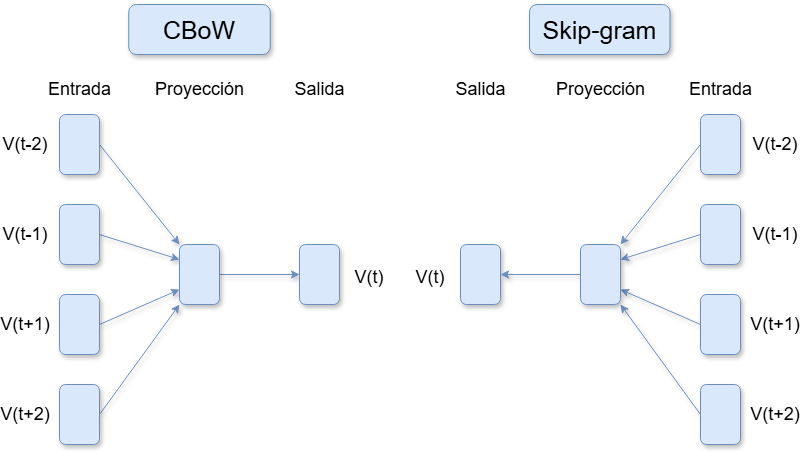
\includegraphics[width=1\textwidth]{imagenes/word2vec.drawio.png}
    \caption{Arquitecturas de Word2Vec. La arquitectura CBOW predice la palabra actual en función del contexto, mientras que Skip-gram predice las palabras circundantes dada la palabra actual.}
    \label{fig:word2vec}
\end{figure}

\sidetext{CBOW}

El modelo CBOW predice la palabra objetivo a partir de las palabras de contexto circundantes. Dicho de otro modo, utiliza las palabras del entorno para predecir la palabra en particular. Este modelo toma todas las palabras de contexto, las procesa y usa el vector resultante para predecir la palabra objetivo. Este modelo resulta beneficioso para tareas de índole más sintáctica, acompañado por un costo de computo menor. \parencite{mikolov2013efficientestimationwordrepresentations}

\sidetext{Skip-gram}

El modelo Skip-Gram predice las palabras de contexto circundante a partir de una palabra objetivo. En resumen, utiliza una sola palabra para predecir su contexto circundante.
Este modelo funciona bien para tareas más semánticas. \parencite{mikolov2013efficientestimationwordrepresentations} Sin embargo, es computacionalmente más costoso que el modelo CBOW debido a su tarea de predecir múltiples palabras de contexto.

\sidetext{Entrenamiento}

Cada palabra en el corpus se representa inicialmente como un vector de alta dimensión, previamente fijado con valores aleatorios. Estos vectores sirven como punto de partida para el proceso de entrenamiento. A medida que avanza el entrenamiento, estos vectores se actualizan en función de la función objetivo del modelo. En consecuencia, estos se posicionan más cerca entre sí en el espacio vectorial a los vectores de palabras que aparecen en contextos similares.

Otro aspecto crítico en el entrenamiento de Word2Vec es la elección del tamaño de la ventana. La ventana actúa como una ventana deslizante que pasa sobre el texto y determina qué palabras se analizan en el contexto de una palabra objetivo. Las palabras dentro de la ventana se consideran parte del contexto, mientras que las que están fuera se ignoran. La elección del tamaño de la ventana genera efectos distintos en los vectores. Un tamaño de ventana más pequeño permite que el modelo realice un aprendizaje más enfocado en la palabra objetivo, mientras que un tamaño de ventana más grande ayuda al modelo a comprender el contexto en el que fue utilizada la palabra objetivo mucho más en detalle. \parencite{levy2014} Sin embargo, un tamaño de ventana más grande aumenta la complejidad computacional del modelo, ya que se deben procesar más palabras de contexto para cada palabra objetivo.

Además, otra de las características que define a Word2Vec es la utilización de \textit{Negative Sampling}, \parencite{mikolov2013distributedrepresentationswordsphrases} el cual aborda el problema de la eficiencia computacional actualizando solo un pequeño porcentaje de los pesos del modelo en cada paso en lugar de todos ellos. Esto se logra seleccionando un pequeño número de palabras “negativas” (palabras que no están en el contexto) para actualizarlas en cada palabra objetivo.

Por último, en el modelo se realiza un submuestreo de palabras frecuentes, el cual ayuda a mejorar la calidad de los vectores de palabras. \parencite{mikolov2013distributedrepresentationswordsphrases} La idea básica es reducir el impacto de las palabras de alta frecuencia en el proceso de entrenamiento, ya que a menudo contienen información menos significativa en comparación con las palabras no frecuentes.

Al descartar aleatoriamente algunas instancias de palabras frecuentes, el modelo se ve obligado a centrarse más en las palabras raras, lo que lleva a vectores de palabras más equilibrados y con información más relevante.

\subsection{Modelos de Lenguaje}

A los \textit{embeddings} no solo los podemos encontrar como resultado de arquitecturas como Word2Vec, sino también como partes clave de otros modelos cuyo objetivo es distinto al de generar una serie de vectores de palabras; tal es el caso de algunos modelos de lenguaje, como el de la arquitectura AWD-LSTM.

Yendo más en detalle, un modelo de lenguaje es un tipo de modelo de aprendizaje automático entrenado para establecer una distribución de probabilidad sobre las palabras. Básicamente, un modelo intenta predecir la siguiente palabra más adecuada para llenar un espacio en blanco en una oración o frase, basándose en el contexto del texto dado.

\begin{figure}[H]
    \centering
    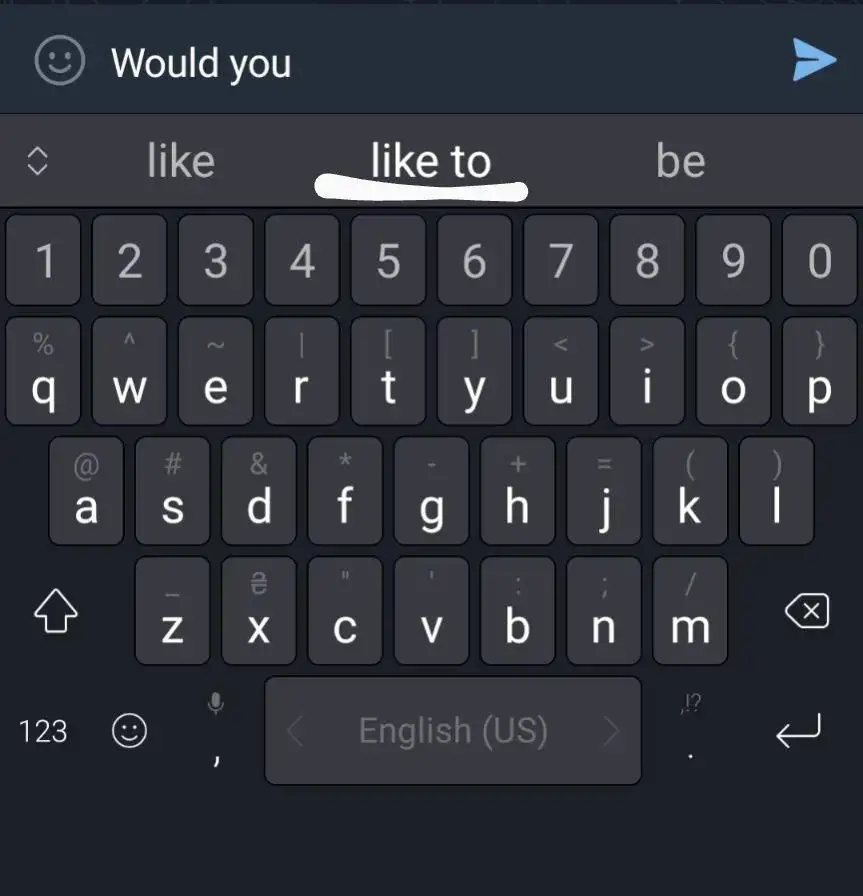
\includegraphics[width=0.5\textwidth]{imagenes/autocompletado_celular.jpg}
    \caption{Los modelos de lenguaje se utilizan en una variedad de tareas de NLP, como el reconocimiento de voz, el autocompletado de textos y la creación de resúmenes de textos.}
    \label{fig:nlp}
\end{figure}

Son un componente fundamental en el ámbito del NLP porque permiten que las máquinas comprendan, generen y analicen el lenguaje humano. Se entrenan principalmente utilizando grandes corpus de texto. Los modelos luego utilizan los patrones que aprenden de estos datos de entrenamiento para predecir la siguiente palabra en una oración o generar nuevo texto que sea gramaticalmente correcto y semánticamente coherente.

Existen diferentes tipos de Modelos de Lenguaje, los cuales se pueden clasificar en dos categorías: \textbf{modelos estadísticos} y modelos basados en \textbf{redes neuronales profundas}.

Por un lado, los modelos estadísticos de lenguaje son un tipo de modelo que utilizan patrones estadísticos en los datos para hacer predicciones sobre la probabilidad de secuencias específicas de palabras. Por ejemplo, un enfoque básico para construir un modelo de lenguaje probabilístico es la utilización de n-gramas.

Por otro lado, los modelos de lenguaje neuronales, como su nombre indica, utilizan redes neuronales para predecir la probabilidad de una secuencia de palabras. Estos modelos se entrenan con un gran corpus de datos de texto y cumplen el objetivo de predecir palabras dado un contexto al minimizar una función de costo.

\begin{figure}[H]
    \centering
    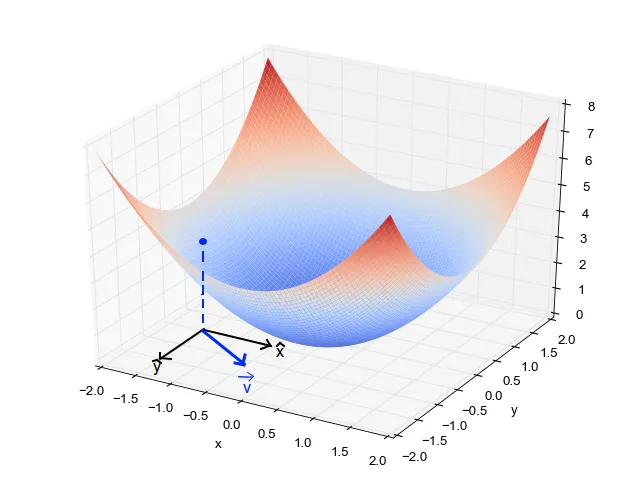
\includegraphics[width=0.8\textwidth]{imagenes/function.jpg}
    \caption{La idea general de los modelos basados en redes neuronales es minimizar una función de costo generada a partir de los pesos de la red. Para esto se calcula el gradiente de la función en un punto, o sea la pendiente de la tangente a la función de coste. Este gradiente puede ser calculado de a batches o de a una entrada a la vez, o sea de manera estocástica.}
    \label{fig:gradiente}
\end{figure}

Una vez entrenados estos modelos, los mismos permiten captar mejor dependencias de largo alcance entre palabras que con los modelos estadísticos tradicionales. \parencite{Wang2017ngram} Por ejemplo, al utilizar un modelo estadístico basado en n-gramas, el contexto que presenta el modelo es limitado, mientras que los modelos basados en redes neuronales presentan diversidad de estrategias para poder recordar contextos lejanos a lo largo del entrenamiento. Esta es la razón por la cual nos decantamos por ellas. Una de las arquitecturas más reconocidas que utiliza estas estrategias son las Redes neuronales recurrentes (RNNs).

\subsubsection{Redes neuronales recurrentes}

Una red neuronal recurrente, o RNN, es una red neuronal profunda entrenada con datos secuenciales o de series temporales para crear un modelo de aprendizaje automático que pueda hacer predicciones o conclusiones basadas en estas mismas.

\begin{figure}[H]
    \centering
    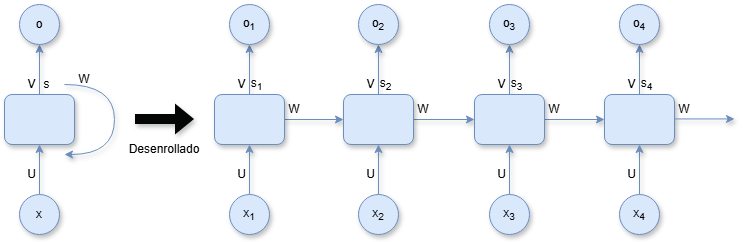
\includegraphics[width=1\textwidth]{imagenes/RNN.drawio.png}
    \caption{Diagrama de una Red neuronal recurrente mostrando su versión compacta a la izquierda y su versión desenrollada a la derecha, ilustrando cómo la red se expande a lo largo del tiempo para procesar secuencias de datos.}
    \label{fig:rnn}
\end{figure}

Se distinguen por su “memoria”, ya que toman información de entradas anteriores para influir en la entrada y salida actuales. Mientras que las redes neuronales profundas tradicionales suponen que las entradas y salidas son independientes entre sí, la salida de las redes neuronales recurrentes depende de los elementos anteriores dentro de la secuencia. Incluso existen tipos de RNNs cuya salida actual no solo se ve influenciada por los resultados anteriores sino también por los resultados futuros.

Otra característica distintiva de las redes recurrentes es que comparten parámetros en cada capa de la red. Mientras que las redes tradicionales tienen diferentes pesos en cada nodo, las redes neuronales recurrentes comparten pesos en cada capa de la misma. Dichos pesos se ajustan a través de los procesos de \textit{backpropagation} y descenso por el gradiente para facilitar el aprendizaje.

Las redes neuronales recurrentes utilizan algoritmos de \textit{backpropagation} a través del tiempo (BPTT, de sus siglas en inglés) para determinar los gradientes, lo cual es ligeramente diferente del algoritmo tradicional, ya que es específico para datos secuenciales. Los principios de BPTT son los mismos que los de \textit{backpropagation} tradicional, donde el modelo se entrena calculando errores desde su capa de salida hacia la capa de entrada. Estos cálculos permiten ajustar y adaptar los parámetros del modelo adecuadamente. La diferencia con el enfoque tradicional es que BPTT suma los errores en cada paso temporal, mientras que las redes normales no necesitan hacerlo, ya que no comparten parámetros entre las capas.

Este tipo de redes, sin embargo, se ven afectadas por diversas cuestiones. Una de ellas, aunque no de manera tan tajante como puede ser en el caso de los modelos basados en n-gramas, es la incapacidad de recordar dependencias a largo plazo; es decir, si el estado anterior que influye en la predicción actual no está en el pasado reciente, el modelo RNN puede no ser capaz de predecir correctamente el estado actual.

Por ejemplo, supongamos que queremos predecir las palabras en la siguiente oración:

\begin{center}
    ...\hlred{Alicia es alérgica a} \hlorange{los frutos secos. Ella} \hlyellow{no puede comer nueces}...
\end{center}

El contexto de una alergia a los frutos secos nos ayuda a anticipar que el alimento que no se puede comer contiene frutos secos. Sin embargo, si ese contexto se mencionara varias oraciones antes, sería difícil para la RNN inferir esa información, debido a su falta de capacidad para asociar relaciones entre oraciones muy distantes.

A su vez, se considera que las RNNs, las cuales en su mayoría dividen la información del dataset en batches de tamaño fijo,  presentan algunos inconvenientes a la hora de manejar la información de entrenamiento de manera eficiente. Esto se debe a que al utilizar un tamaño fijo para el batch, independientemente en la época que esté del entrenamiento, siempre van a existir un grupo de elementos del batch los cuales no van a poder aprovecharse de la capacidad recurrente de la red. Por ejemplo, volviendo al caso de la oración anterior, si entrenáramos nuestro modelo con batches de tamaño 4, nos pasaría que palabras como ‘Alicia’, ‘los’ y ‘no’ no se aprovecharían de la información previa a ellas, a pesar de ser esto una pieza clave de las RNN. \parencite{merity2017regularizingoptimizinglstmlanguage}

Al mismo tiempo, durante este proceso, las RNN tienden a enfrentar otros dos problemas, conocidos como \textit{exploding gradients} y \textit{vanishing gradients}. Estos problemas se definen por el tamaño del gradiente. Cuando el gradiente es demasiado pequeño, este mismo sigue disminuyendo hasta que los parámetros de peso se vuelven insignificantes, y en ese punto, el algoritmo deja de aprender. Por otro lado, los gradientes que explotan ocurren cuando el gradiente es demasiado grande, creando un modelo inestable. En este caso, los pesos del modelo crecerán demasiado y eventualmente se llegará a problemas de convergencia.

Una solución utilizada para mitigar estos problemas, especialmente el de los gradientes altos, es la implementación del concepto de \textit{gradient clipping}, el cual se basa en la idea de establecer un límite, el cual si es pasado por el gradiente durante el entrenamiento se procede a reducir proporcionalmente el mismo para evitar que el vector se vuelva demasiado grande. \parencite{pascanu2013difficultytrainingrecurrentneural} A su vez también han surgido otras arquitecturas de modelos de lenguaje que buscan afrontar estos problemas.

\subsubsection{LSTM}

Las LSTMs (proveniente del inglés, \textit{Long Short-Term Memory}) son una serie de arquitecturas populares de RNNs surgidas con el objetivo de solucionar el problema del \textit{exploding gradients} y \textit{vanishing gradients}. Además, con esta arquitectura se busca resolver otros inconvenientes como el de la incapacidad de asociar dependencias a largo plazo. \parencite{lstm}

Para solucionar esto, las redes LSTM introducen un nuevo tipo de células de memoria, distintas a las presentes en las RNNs y capaces de retener información a lo largo de secuencias extensas. Cada célula de memoria presenta tres componentes principales: una puerta de entrada, una puerta de olvido y una puerta de salida. Estas puertas ayudan a regular el flujo de información dentro y fuera de la célula de memoria.

\begin{figure}[H]
    \centering
    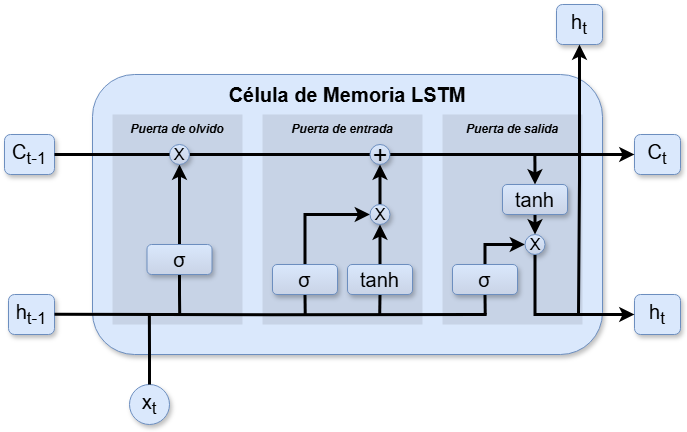
\includegraphics[width=1\textwidth]{imagenes/LSTM.png}
    \caption{Diagrama de una LSTM junto a sus puertas. Las LSTM utilizan estas para regular el flujo de información, lo que les permite aprender dependencias a largo plazo en los datos, haciéndolas particularmente efectivas para tareas que involucran datos secuenciales como la predicción de series temporales, el procesamiento del lenguaje natural, el reconocimiento de voz, y más.}
    \label{fig:lstm}
\end{figure}

\begin{itemize}
    \item \textbf{La puerta de entrada} determina cuánta de la nueva información debe almacenarse en la célula de memoria. Toma la entrada actual y el estado oculto anterior como entradas, y genera un valor entre 0 y 1 para cada elemento de la célula de memoria.
    \item \textbf{La puerta de olvido} decide qué información debe descartarse de la célula de memoria. Al igual que la puerta de entrada, toma la entrada actual y el estado oculto anterior y emite un valor entre 0 y 1. Un valor de 0 significa que la información se ignora, mientras que un valor de 1 indica que se retiene.
    \item \textbf{La puerta de salida} controla cuánta de la información de la célula de memoria debe usarse para calcular el estado oculto. También toma la entrada actual y el estado oculto anterior como entradas y emite un valor entre 0 y 1 para cada elemento de la célula de memoria.
\end{itemize}

Al controlar y memorizar información a lo largo de secuencias largas, las LSTM pueden mitigar los problemas de \textit{exploding gradients} y \textit{vanishing gradients}, permitiendo un entrenamiento más efectivo y una mejor captura de patrones a largo plazo en los datos secuenciales.

Durante los años, muchas arquitecturas han florecido utilizando a las LSTM como base, ya sea como motivación o literalmente. Por ejemplo, una de ellas son las GRU, o \textit{Gated Recurrent Units} de sus siglas en inglés, las cuales tenían como objetivo presentar una alternativa que pudiera solucionar los problemas resueltos por las LSTM, con la ventaja de tener un diseño más simple y una complejidad computacional mucho menor. Esto lo lograban, entre otras cosas, condensando el trabajo de las compuertas de entrada y olvido de la LSTM en una sola compuerta llamada compuerta de actualización. \parencite{chung2014empiricalevaluationgatedrecurrent} Sin embargo, si dejamos de lado la rapidez para entrenar los modelos, las GRU generan peores resultados que las LSTMs fuera de datasets pequeños. \parencite{lstmandgru}

\subsubsection{AWD-LSTM}

\label{sec:awd-lstm}

Otro ejemplo de modelo de lenguaje basado en LSTMs es la AWD-LSTM (de sus siglas en inglés, \textit{ASGD Weight-Dropped LSTM}). A diferencia de la arquitectura LSTM básica, la AWD-LSTM implementa varias técnicas de regularización a lo largo de su red neuronal, con el objetivo de mejorar la capacidad predictiva del modelo, especialmente en la capacidad del modelo para poder generalizar. Además, estas técnicas mejoran la estabilidad del modelo, ya que reducen la probabilidad de sobreajuste del mismo.

\begin{figure}[H]
    \centering
    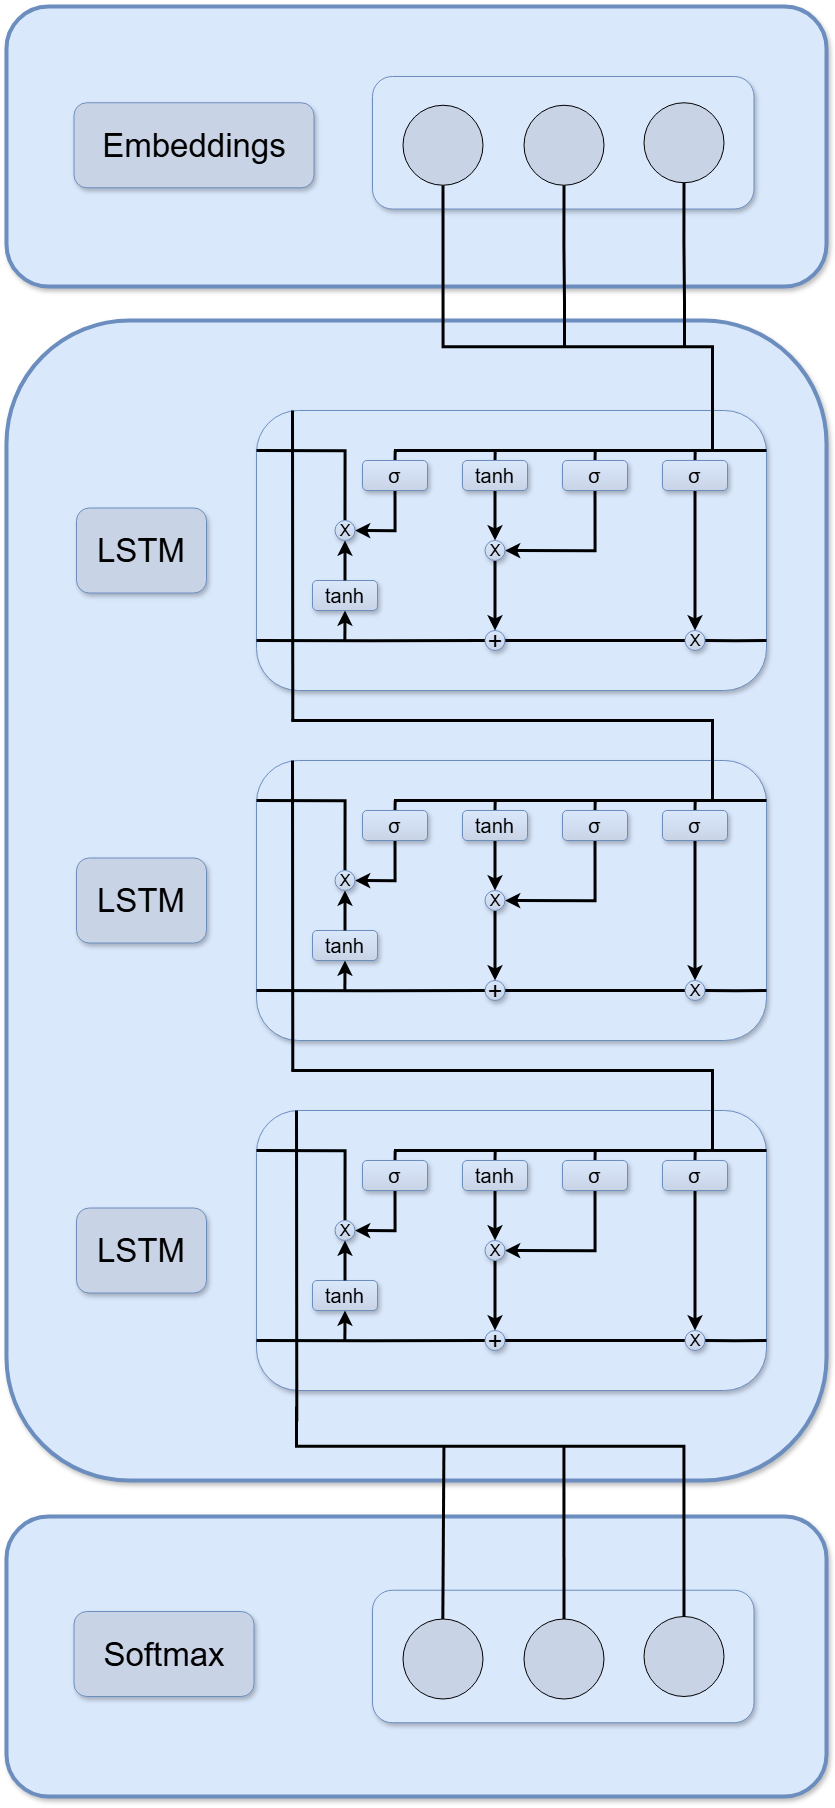
\includegraphics[width=0.42\textwidth]{imagenes/AWD-LSTM.drawio.png}
    \caption{Estructura clásica de un modelo basado en AWD-LSTM. El mismo presenta una capa de \textit{embeddings}, por el cual la entrada pasará y verá sus palabras transformadas en vectores de palabras. Unas 3 células LSTM y una capa softmax la cual permite obtener la distribución de probabilidades para la siguiente palabra del texto dado el vocabulario.}
    \label{fig:awd-lstm}
\end{figure}

Muchas de estas técnicas de regularización están asociadas a la aplicación de \textit{dropout} en porcentajes distintos en distintas partes de la red neuronal. Estas partes en concreto son:

\begin{itemize}
    \item En la capa de \textit{embeddings}, los pesos de algunas palabras dentro del vocabulario de la capa son desactivados.
    \item Luego de la capa de \textit{embeddings}, una vez obtenidos los \textit{embeddings} de todas las palabras del texto de entrada, ciertos pesos de los vectores son desactivados de manera aleatoria.
    \item Previo al ingresar a cada celda LSTM.
    \item Dentro de cada una de las celdas LSTM.
    \item Al finalizar la activación de la última celda.
\end{itemize}

Adicionalmente, la arquitectura introduce un algoritmo de optimización nuevo, llamado NT-ASGD (de sus siglas \textit{Non-monotonically Triggered Averaged Stochastic Gradient Descent}). En resumen, se implementa un algoritmo parecido al de descenso por el gradiente estocástico, con la diferencia de que los pesos de la red no se ven afectados solamente por el gradiente actual, sino por el promedio de los últimos n gradientes, donde n es un hiperparámetro. Además, este promedio no se realiza a partir del primer batch de entrada, sino que el algoritmo actúa como un descenso por el gradiente estocástico normal hasta que el modelo empeora o se estanca durante varias entradas seguidas, a partir del cual se empieza a calcular el gradiente final en base al promedio de los anteriores hasta finalizar el entrenamiento.

Asimismo, anteriormente habíamos mencionado que las RNNs podían llegar a no ser 100\% eficientes en el uso del dataset de entrenamiento, debido a que, en el caso de las tareas de predicción de texto, existen algunas palabras que no aprovechan la capacidad recurrente de la red si se utiliza un tamaño de batch fijo durante el entrenamiento. Este problema es atacado por la AWD-LSTM variando el tamaño del batch que se utiliza en cada época. En particular esta variación la realiza partiendo de un tamaño base, el cual llamaremos $seq$. En un primer paso, se elige como valor intermedio con probabilidad $p$ a este valor $seq$ y con probabilidad $1-p$ a $\frac{seq}{2}$, con $p$ un valor muy cercano a 1. Esto se hace para aumentar el rango de valores usados durante el entrenamiento. Para finalizar, se selecciona el tamaño de batch final a partir de una distribución normal con media en ese valor intermedio y un desvío estándar. De esta manera, se aprovecha mucho más la capacidad recurrente de la AWD-LSTM.

Por último, el \textit{learning rate} del modelo es re-escalado dependiendo del tamaño de batch resultante, ya que se ha encontrado una tendencia a favorecer a las oraciones más cortas durante el entrenamiento si se utiliza un tamaño de batch variable junto a un \textit{learning rate} fijo. \parencite{merity2017regularizingoptimizinglstmlanguage}

Debido a estas mejoras introducidas por esta arquitectura y porque fue una de las más populares previo al surgimiento de otros modelos como los \textit{transformers}, decidimos tomar a la AWD-LSTM como nuestro eje principal en ese trabajo.

\subsubsection{Evaluación}

Una vez se tiene elegido el tipo de arquitectura de modelos de lenguaje que se utilizara para llevar a cabo nuestro propósito, es lógico preguntarse de qué manera podemos evaluar nuestros modelos para ver si se comportan de manera satisfactoria y son capaces de comprender el lenguaje humano.

Para esto, fuera de las típicas métricas utilizadas para evaluar modelos de aprendizaje automático como el \textit{Accuracy} o el \textit{F1 Score}, existen otras, como la \textit{Perplexity}, la cual es considerada como una medida utilizada para cuantificar la incertidumbre asociado con una distribución de probabilidad. Esta métrica a lo largo de los años se ha utilizado como una manera de evaluar distintos modelos de lenguaje. \parencite{merity2017regularizingoptimizinglstmlanguage}

Yendo más en detalle, esta métrica se define como la exponenciación de la entropía de una distribución de probabilidad. Se puede expresar como:

\[
PP(W) = 2^{H(W)}
\]

donde el $H(W)$ es la entropía del modelo con respecto a la secuencia de palabras $W$. Un nivel de \textit{perplexity} más bajo indica un mejor modelo predictivo, ya que implica que el modelo tiene más confianza en sus predicciones. Por el contrario, un nivel de \textit{perplexity} más alto sugiere una mayor incertidumbre y predicciones menos efectivas.

\section{Movimientos oculares durante la lectura}

La lectura se puede considerar como un desarrollo relativamente reciente en la historia de la humanidad, existiendo sólo desde hace unos pocos miles de años. \parencite{ImmordinoYangDeacon2007} Sin embargo, se ha convertido en una habilidad esencial en la vida moderna, que se desarrolla a lo largo de años de exposición, instrucción formal y práctica.
Una buena habilidad de lectura es fundamental para el logro académico (para una discusión, ver \textcite{Renadya}), y para los estudiantes de un segundo idioma, la lectura es una puerta de entrada para aprender nuevo vocabulario, más lenguaje coloquial y nuevas construcciones gramaticales. \parencite{wilkinson}

Sabemos que para los lectores el objetivo principal es identificar palabras, comprender su significado e integrarlas en su comprensión progresiva de una oración y/o de un discurso más amplio. Sin embargo, ¿Qué ocurre exactamente cuando leemos? ¿Cómo se mueven nuestros ojos?

Tal y como menciona \textcite{Brown1895}, nuestros ojos a la hora de leer se asemejan al movimiento del segundero dentro de un reloj, se realiza un tirón y una pequeña pausa, luego otro tirón, y así sucesivamente; solo que nuestros ojos no son tan regulares, los tirones a veces tienen una amplitud mayor o menor, y las pausas varían en duración, aunque, a menos que hagamos un esfuerzo, siempre son breves. Durante los tirones prácticamente no vemos nada, por lo que no tenemos ante nosotros un panorama en movimiento, sino una serie de imágenes fijas que se suceden rápidamente.

Estos “tirones” del ojo — en otras palabras, sus movimientos — son lo que comúnmente denominamos sacadas. El intervalo entre los movimientos de los ojos, cuando estos se detienen, se llama fijación. Ambos son un tipo de respuesta fisiológica automática, lo que significa que no están bajo nuestro control consciente. \parencite{Rayner2012} Cualquier secuencia completa de estos dos se denomina como un \textit{scanpath}. Sin embargo, al leer, las sacadas no siempre mueven el ojo hacia adelante en el texto. Aproximadamente entre el 10 y el 15 por ciento de las veces, los lectores mueven los ojos hacia atrás (regresan) a secciones del texto previamente vistas. Estos movimientos hacia atrás se conocen como regresiones. Las regresiones pueden ser cortas o largas. Las regresiones cortas suelen deberse a un exceso de movimiento sobre el objetivo. Por otro lado, las regresiones largas son atribuidas comúnmente a la dificultad del texto leído, que puede deberse a diversos factores.

Básicamente, cuando leemos o miramos una escena o imagen, nuestros ojos se detienen para procesar la información en esa ubicación y luego se mueven a otro punto donde hay otra información disponible. Durante las fijaciones, el sistema cognitivo percibe y procesa la información visual, además de planificar cuándo y hasta dónde mover los ojos a continuación. En la mayoría de las circunstancias normales, durante un movimiento sacádico, los ojos se mueven tan rápido que no obtenemos nueva información visual. \parencite{Rayner2009} Sin embargo, mientras no se codifica nueva información visual durante los movimientos sacádicos, el procesamiento de la información ya percibida previamente continua. \parencite{Irwin1998} \parencite{Irwin1996}

Entonces, ¿de qué manera podría interesar el rastreo y medición de los movimientos oculares de las personas dentro de la lectura? Las fijaciones, los movimientos sacádicos y las regresiones ocurren generalmente de forma “automática”, sin que seamos conscientes de ello. De esta forma, el seguimiento de los movimientos oculares nos ofrece una ventana a un comportamiento en gran medida inconsciente. Además, se ha demostrado que en tareas de procesamiento complejo, como es el caso de la lectura, la ubicación de los ojos proporciona un índice de atención. \parencite{Rayner2009} Esto significa que nuestros ojos indican en qué estamos prestando atención y cuánta energía cognitiva se está invirtiendo para procesar la información en el punto de fijación. Así, la dificultad y la complejidad de lo que miran los ojos influyen en las fijaciones y los movimientos sacádicos. \parencite{CastelhanoRayner2008} Cuando el estímulo es más difícil, aumentan las duraciones de fijación y las regresiones, mientras que el tamaño de los movimientos sacádicos disminuye. Esto significa que, en la lectura, los textos más difíciles provocan fijaciones y regresiones más frecuentes y prolongadas, mientras que los sacádicos se acortan. Al observar escenas o imágenes más densas o complejas, las fijaciones también se alargan y los movimientos sacádicos se acortan.

Estas, en definitiva, son algunas de las razones por las cuales el análisis de movimientos oculares se ha vuelto una de las herramientas más poderosas para estudiar la manera en que la información visual es procesada por la mente humana y una de las herramientas más estándares a la hora de realizar estudios sobre lectura en los campos de la psicolingüística, la psicología cognitiva y la lingüística aplicada. \parencite[p. 1474]{Rayner2009} Sin embargo, cabe aclarar que todas estas ventajas brindadas por el análisis de los movimientos oculares se apoyan en gran medida en lo que se conoce como la hipótesis ojo-mente, la cual afirma que hay una estrecha relación entre los movimientos del ojo y el procesamiento cognitivo dentro de nuestro cerebro a la hora de leer. \parencite{JustCarpenter1980} A su vez, esta hipótesis se basa en dos ideas subyacentes:

\begin{enumerate}
    \item Primero, está la suposición de que lo que se está fijando es lo que se está considerando. Esto significa que cuando los ojos se fijan en una palabra “x”, el cerebro está trabajando para descifrar y entender esta palabra y no otra palabra “z” que apareció tres palabras antes. Es decir, los lectores intentan interpretar las palabras a medida que las encuentran. No obstante, esta suposición termina resultando ser, aunque acertada, algo simplista. \parencite{EhrlichRayner1983} Por ejemplo, en una oración como “Maria vendió su caballo a José porque ella decidió dejar de montar”, cuando los ojos se posan en la palabra “ella”, para interpretarla, el cerebro necesita considerar entidades previamente encontradas que podrían ser referentes potenciales del pronombre. Así, cuando los ojos se detienen en “ella”, la mente está trabajando en esta palabra; sin embargo, también considera elementos previos de la oración que podrían ser referentes potenciales (por ejemplo, “Maria”).
    \item La segunda parte, por otra parte, estipula que la cantidad de tiempo dedicado a fijar un elemento o región refleja el esfuerzo cognitivo necesario para procesarlo. Esto significa que fijaciones más largas y frecuentes indican un mayor esfuerzo de procesamiento, y las fijaciones más breves y/o los saltos indican un menor esfuerzo de procesamiento. Además, es importante aclarar que estos tiempos deben tomarse en términos relativos: una mayor o menor duración y un mayor o menor esfuerzo de procesamiento deben compararse con algo. En general, el esfuerzo cognitivo se decide asociar a una región de interés en particular (conocida como ROI, de sus siglas en inglés)
\end{enumerate}

\subsection{Métricas asociadas a movimientos oculares}

\label{subsec:metricas_movimientos}

Habiendo previamente mencionado todas las ventajas de la utilización de movimientos oculares para obtener información sobre el comportamiento inconsciente de las personas a la hora de leer, parecería lógico preguntarse de qué manera se puede extraer esta información.

A partir de esto, la tecnología de seguimiento ocular nos permite indicar, entre otras cosas, dónde se posan los ojos de las personas, cuántas veces se posan en esa posición o región (conteo de fijaciones) y cuánto dura cada fijación (duración de fijación), además de medir la duración y la longitud de los movimientos sacádicos. Estas medidas se toman en experimentos utilizando el equipamiento adecuado, dividiendo los mismos en distintas pruebas, donde el equipamiento va recolectando información sobre los movimientos oculares de un sujeto a medida que este va realizando la lectura de un corpus de texto.

Ahora, dado que las fijaciones (y específicamente la duración de las mismas) son más sensibles a los factores lingüísticos que los movimientos sacádicos \parencite{StaubRayner2007}, estas tienden a ser las métricas que más nos interesan en estudios basados en textos. Estas métricas se clasifican en “tempranas”, “intermedias” o “tardías” y se entiende que reflejan diferentes etapas del procesamiento de la lectura. Las medidas tempranas se consideran principalmente como un reflejo de procesos automáticos de reconocimiento de palabras y acceso léxico, mientras que las medidas tardías tienden a reflejar procesos más conscientes, controlados y estratégicos. (\cite{Altarriba1996}; \cite{Inhoff1984}; \cite{Paterson1999}; \cite{StaubRayner2007})

\begin{figure}[H]
    \centering
    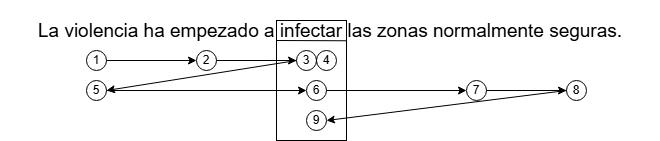
\includegraphics[width=1\textwidth]{imagenes/scanpath.png}
    \caption{Ejemplo de scanpath. Cada círculo debajo de una palabra indica una fijación en el orden el cual fue hecha mientras que las flechas indican las sacadas realizadas. En este caso la palabra crítica tenida en cuenta es “infectar”.}
    \label{fig:scanpath}
\end{figure}

\subsubsection{Métricas tempranas}

Cada una de estas métricas puede considerarse como un índice de acceso léxico, o de qué tan fácilmente se reconoce y se recupera la palabra del léxico mental. Algunos factores que se sabe que afectan estas métricas incluyen la frecuencia y familiaridad de la palabra, la ambigüedad de significado, la predictibilidad y la asociación semántica.

\begin{itemize}
    \item \textit{Skipping Rate}: Se utiliza para determinar la proporción de palabras que no reciben fijación, o sea las palabras que son salteadas durante la primera pasada de lectura. Esta métrica se suele reportar como una probabilidad (o porcentaje) y se calcula como el número total de pruebas en los que la palabra se omitió durante la primera pasada de lectura dividido el número total de pruebas. Por ejemplo, en el scanpath de arriba vemos que la palabra crítica no fue salteada, por lo que esta prueba contribuiría a la cantidad total de pruebas pero no al numerador de la división.
    \item \textit{First Fixation Duration}: Ó FFD proveniente de su acrónimo en inglés, se refiere al tiempo de la primera fijación realizada en una palabra o región de interés. En el caso de ejemplo se consideraría solamente el tiempo de la fijación número 3.
    \item \textit{Single Fixation Duration}: Métrica muy parecida a la anterior, con la diferencia de que solo se tienen en cuenta las pruebas donde se ha realizado una sola fijación sobre la palabra en cuestión o ROI. En el caso de la palabra crítica en el ejemplo no se vería contada al presentar más de una fijación.
    \item \textit{First Pass Reading Time}: También conocida como \textit{Gaze Duration} o FPRT, considera todas las fijaciones hechas en una palabra o ROI antes de que la mirada salga (ya sea a la izquierda o a la derecha) de la misma. Dentro del ejemplo presentado, la suma se realizaría entre los tiempos de las fijaciones 3 y 4.
\end{itemize}

\subsubsection{Métricas intermedias}

Existen métricas que son difíciles de clasificar como tempranas o tardías, como las relacionadas a las regresiones dentro de la lectura, ya que pueden indicar dependiendo de cómo se las utilice como dificultad al encontrar un elemento por primera vez, así como el tiempo posterior necesario para superar esa dificultad. \parencite{CliftonStaubRayner2007}

\begin{itemize}
    \item \textit{Regression Path Duration}: también conocida como \textit{go past time}, es una medida del tiempo dedicado a la palabra en sí y a cualquier parte anterior de la oración antes de que el lector avance más allá de la palabra crítica hacia la derecha. También se puede medir una métrica parecida en términos de cantidad o como un porcentaje, es decir, cuántas pruebas tuvieron una regresión dentro del ROI. Volviendo al ejemplo, la métrica en este caso estaría compuesta por la suma de la duración de las fijaciones 3, 4, 5 y 6.
\end{itemize}

\subsubsection{Métricas tardías}

Las medidas tardías pueden no reflejar factores puramente léxicos y estar más influenciadas por propiedades contextuales, sintácticas o de nivel de discurso de lo que se está leyendo. Por ejemplo, la ambigüedad sintáctica puede llevar a fijaciones más prolongadas en una palabra o región crítica, así como a más regresiones al contexto anterior a medida que el lector se ve obligado a reevaluar el análisis inicial. \parencite{FrazierRayner1982}

\begin{itemize}
    \item \textit{Total Reading Time}: Es la suma de todas las fijaciones realizadas en una palabra o ROI durante un ensayo. En el ejemplo, el \textit{Total Reading Time} de la palabra crítica sería la suma de las fijaciones 3, 4, 6 y 9.
    \item \textit{Re-reading Time}: Existen diferentes definiciones de la misma dentro de la literatura. Una de ellas se calcula a partir de la resta entre dos métricas anteriormente mencionadas, el \textit{Regression Path Duration} menos el \textit{First Pass Reading Time}. Abstrayendo al caso en particular, haciendo la resta de las dos métricas previas se tendría que el \textit{Re-reading Time} es la suma de la fijación 5 y 6.
    \item \textit{Second Pass Reading Time}: Se define como la suma de todas las fijaciones dentro de un ROI luego de haber abandonado la región de interés por primera vez. En el caso de ejemplo, la suma se realizaría entre las fijaciones 6 y 9.
    \item \textit{Fixation Count}: Cantidad de fijaciones realizadas sobre un ROI. En este caso, un total de 4 fijaciones sobre la palabra crítica.
\end{itemize}

Es fundamental recordar que las medidas no son independientes entre sí: \textit{First Fixation Duration} es parte de \textit{First Pass Reading Time}, que a su vez es parte de \textit{Total Reading Time}. De manera similar, \textit{Total Reading Time} y \textit{Fixation Count} generalmente están altamente correlacionados. Por lo tanto, a la hora de utilizar estas métricas, el objetivo debe ser analizar una gama de medidas para investigar el patrón general, y si un efecto sólo aparece en una de nuestras medidas, esto debe interpretarse con precaución.

\section{Movimientos oculares en NLP}

A medida que los modelos de NLP se vuelven cada vez más frecuentes en la sociedad, los investigadores han visto la necesidad de buscar maneras de cómo mejorar estos modelos, por ejemplo aprovechando información recopilada de manera pasiva de los lectores humanos, como las señales de movimientos oculares.

Esto genera que recientemente los movimientos oculares hayan incursionado en el campo de NLP, a partir de las relaciones existentes entre la duración de la mirada sobre las palabras (\textit{gaze duration}) y la capacidad de predecirlas (\cite{Rayner1998}, \cite{Reinhold2006}). Particularmente, se realizaron análisis sobre los modelos del lenguaje en conjunto a datos de MO para capturar la relación entre ellos (\cite{Bianchi2020}, \cite{Hofmann2017}), revelando información sobre la influencia de otras variables (como la frecuencia de la palabra) y permitiendo obtener una mejor comprensión de qué mecanismos actúan en el cerebro en determinado momento. Otros trabajos se han enfocado en la incorporación de los datos de MO para mejorar los modelos del estado del arte, en campos como el etiquetado de palabras (\textit{Part of Speech Tagging}) \parencite{barrett-etal-2016-weakly}, compresión de oraciones (\textit{Sentence compression}) \parencite{klerke2016improvingsentencecompressionlearning}, traducción automática (\textit{Machine translation}) \parencite{sajjad-etal-2016-eyes}, análisis de sentimiento (\textit{Sentiment analysis}) \parencite{mishra2017} y reconocimiento de entidades nombradas (\textit{Named-entity Recognition}). \parencite{hollenstein2019} En todos los casos, se observaron mejoras frente a los modelos que no tenían en consideración estos datos.

Curiosamente, la manera de incorporar esta información cognitiva a los modelos de NLP varía según el caso, por ejemplo existen casos en donde la información es concatenada a los \textit{embeddings} del modelo \parencite{hollenstein2019}, mientras que en otros casos se aprovecha de un tipo de entrenamiento conocido como aprendizaje multitarea. \parencite{klerke2016improvingsentencecompressionlearning}

\subsection{Aprendizaje Multitarea}

¿En qué consiste entonces esta técnica? El aprendizaje multitarea (MTL, por sus siglas en inglés) consiste en entrenar una red neuronal para ejecutar múltiples tareas compartiendo algunas de las capas y parámetros de la red entre las mismas. El objetivo es mejorar la capacidad de generalización del modelo aprovechando la información compartida entre las tareas, prediciendo varias cosas a la vez. \parencite{Caruana1997}

\begin{figure}[H]
    \centering
    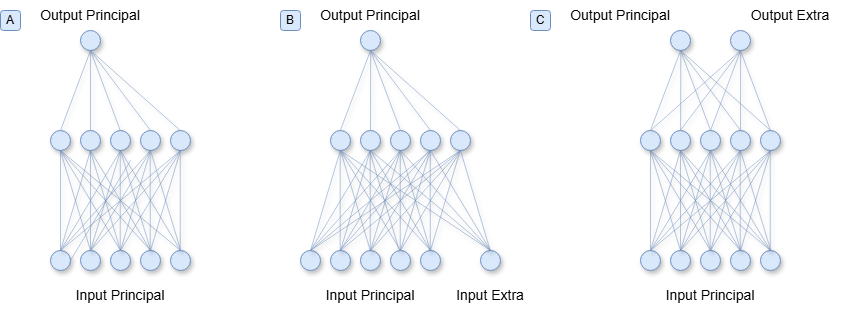
\includegraphics[width=1\textwidth]{imagenes/multitarea.png}
    \caption{Aprendizaje multitarea como es descrito por \textcite{Caruana1997}. La red neuronal A es una red estándar la cual no utiliza ningún tipo de información extra. Por otro lado la red B incorpora comportamiento extra añadiendolo como input de la red. En el caso de la red C se aplica el aprendizaje multitarea: el comportamiento extra es añadido como output de la red y no como input.}
    \label{fig:multitarea}
\end{figure}

Llevándolo al ámbito de NLP con la utilización de movimientos oculares, el aprendizaje multitarea surge como una oportunidad, ya que al saber que el tiempo dedicado a fijarse en una palabra es un indicador de la atención, forzar al modelo de lenguaje a predecir la duración de la fijación de las palabras actúa como una forma de incorporar la atención (cognitiva) en él. En este trabajo, proponemos incorporar dicha información dentro de los \textit{word embeddings} generados.
